\onecolumn
\chapter{Auswertung}
\label{ch:auswertung}

\section*{Fehlerrechnung}
Für die statistische Auswertung von $n$ Messwerten $x_i$ werden folgende Größen definiert \cite{errorSkript25}:
\begin{align}
    \bar{x} &= \frac{1}{n} \sum_{i=1}^{n} x_i \vphantom{\sqrt{\sum_i^n}^2} && \text{\textcolor{gray}{Arithmetisches Mittel}} \label{eq:arithmetisches_mittel} \\
    \sigma^2 &= \frac{1}{n-1} \sum_{i=1}^{n} (x_i - \bar{x})^2 \vphantom{\sqrt{\sum_i^n}^2} && \text{\textcolor{gray}{Variation}} \label{eq:variation} \\
    \sigma &= \sqrt{\frac{1}{n-1} \sum_{i=1}^{n} (x_i - \bar{x})^2} \vphantom{\sqrt{\sum_i^n}^2} && \text{\textcolor{gray}{Standardabweichung}} \label{eq:standardabweichung} \\
    \Delta \bar{x} &= \frac{\sigma}{\sqrt{n}} = \sqrt{\frac{1}{n(n-1)} \sum_{i=1}^n(\bar x - x_i)^2} \vphantom{\sqrt{\sum_i^n}^2} && \text{\textcolor{gray}{Fehler des Mittelwerts}} \label{eq:fehler_mittelwert} \\
    \Delta f &= \sqrt{\left(\frac{\partial f}{\partial x} \Delta x\right)^2 + \left(\frac{\partial f}{\partial y} \Delta y\right)^2} \vphantom{\sqrt{\sum_i^n}^2} && \text{\textcolor{gray}{Gauß’sches Fehlerfortpflanzungsgesetz für $f(x,y)$}} \label{eq:gauss_fehlfortpflanzung} \\
    \Delta f &= \sqrt{(\Delta x)^2 + (\Delta y)^2} \vphantom{\sqrt{\sum_i^n}^2} && \text{\textcolor{gray}{Fehler für $f = x + y$}} \label{eq:fehler_summe} \\
    \Delta f &= |a| \Delta x \vphantom{\sqrt{\sum_i^n}^2} && \text{\textcolor{gray}{Fehler für $f = ax$}} \label{eq:fehler_proportional} \\
    \frac{\Delta f}{|f|} &= \sqrt{\left(\frac{\Delta x}{x}\right)^2 + \left(\frac{\Delta y}{y}\right)^2} \vphantom{\sqrt{\sum_i^n}^2} && \text{\textcolor{gray}{relativer Fehler für $f = xy$ oder $f = x/y$}} \label{eq:relativer_fehler} \\
    \sigma &= \frac{|a_{lit} - a_{gem}|}{\sqrt{\Delta a_{lit}^2 + \Delta a_{gem}^2}} \vphantom{\sqrt{\sum_i^n}^2} && \text{\textcolor{gray}{Berechnung der signifikanten Abweichung}} \label{eq:signifikante_abweichung}
\end{align}

\twocolumn

% ////////////  Aufgaben Wechsel ////////////
\section{Aufgabe 1: Function Generator}
Hat Spaß gemacht und war witzig :)
\begin{figure} [h!]
    \centering
        
\includegraphics[width=0.35\textwidth]{img/25/memes/signifikante3.pdf}
    \caption{Meme}
\end{figure}

% ////////////  Aufgaben Wechsel ////////////
\section{Aufgabe 2: Analyse der 9 Signale}

Wir wollen die Signale 1 und 2 genauer analisieren. Signale 3 und 4 werden nur kurz beschrieben. Bei Signal 5 wird die Halbwertszeit berechnet. Signale 7 bis 9 werden dann wieder qualitativ beschrieben.
\subsection*{Signal 1}
\begin{figure} [h!]
    \centering
        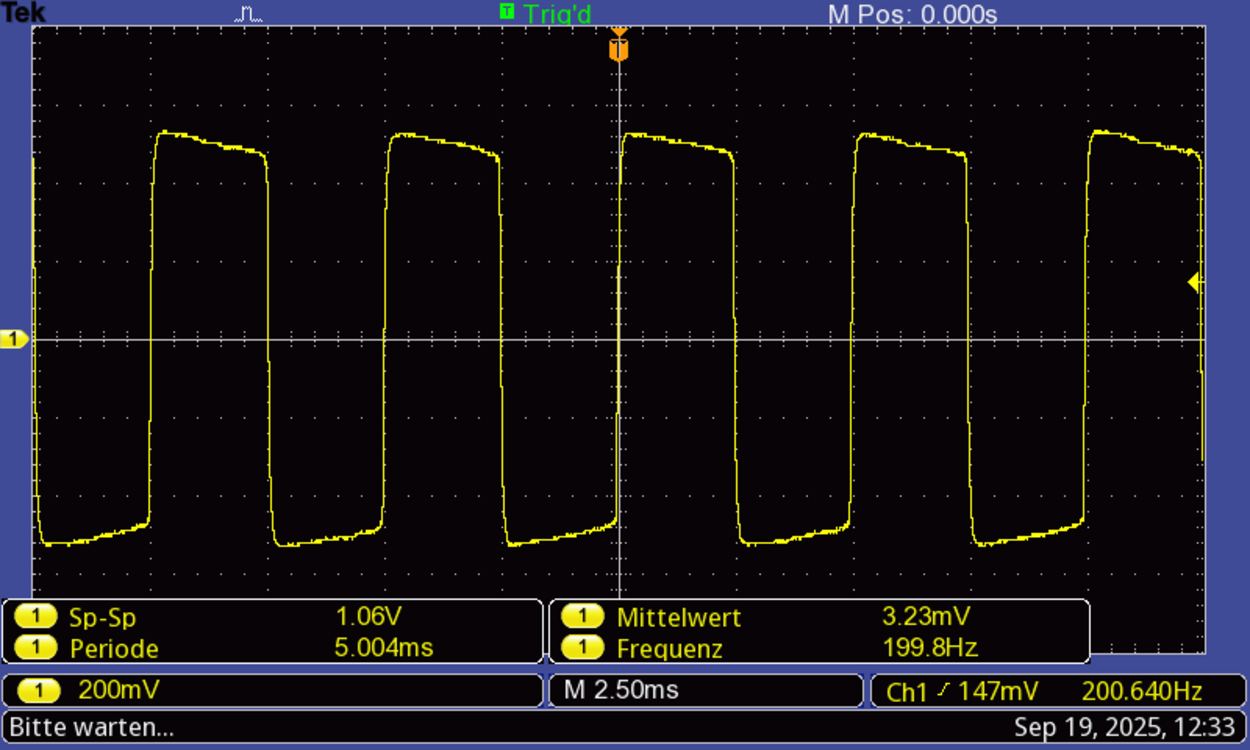
\includegraphics[width=0.45\textwidth]{img/25/Signale2/Signal1-Messwerte.pdf}
    \caption{Signal 1 mit automatischen Messwerten und gesetzem Trigger im AC Modus.}
\end{figure}
Wir mussten zur Vermessung des Signales 1 sowohl manuell mit den Cursorn vermessen und automatisch mit den eingebauten Messfunktionen des Oszilloskopes.
Wir haben dabei eine DIV größe von $200mv \times 2,5ms$ im AC-Modus geahbt und $500mv \times 2,5ms$ im DC-Modus. Aus \hyperref[tab:all_fehler]{Tabelle \ref*{tab:all_fehler}} lassen sich somit die Fehler ablesen beziehungsweise aus den Angaben berechenn lassen zu:
\begin{align}
    &\textcolor{teal}{\Delta V_{AC}} &&= 15\, &&[mV] \\
    &\textcolor{purple}{\Delta V_{DC}} &&= 40\, &&[mV] \\
    &\Delta t &&= 0,16 \, &&[ms].
\end{align}
(Es wurde auf signifikante Stellen gerundet).

In den Tabellen werden die Spalten \textcolor{teal}{Grün} angezeigt, wenn sie in AC gemessen wurden und \textcolor{purple}{Lila}, wenn sie im DC-Modus gemessen wurden. Dies ist nur für die Cursor wichtig.

\begin{figure} [h!]
    \centering
        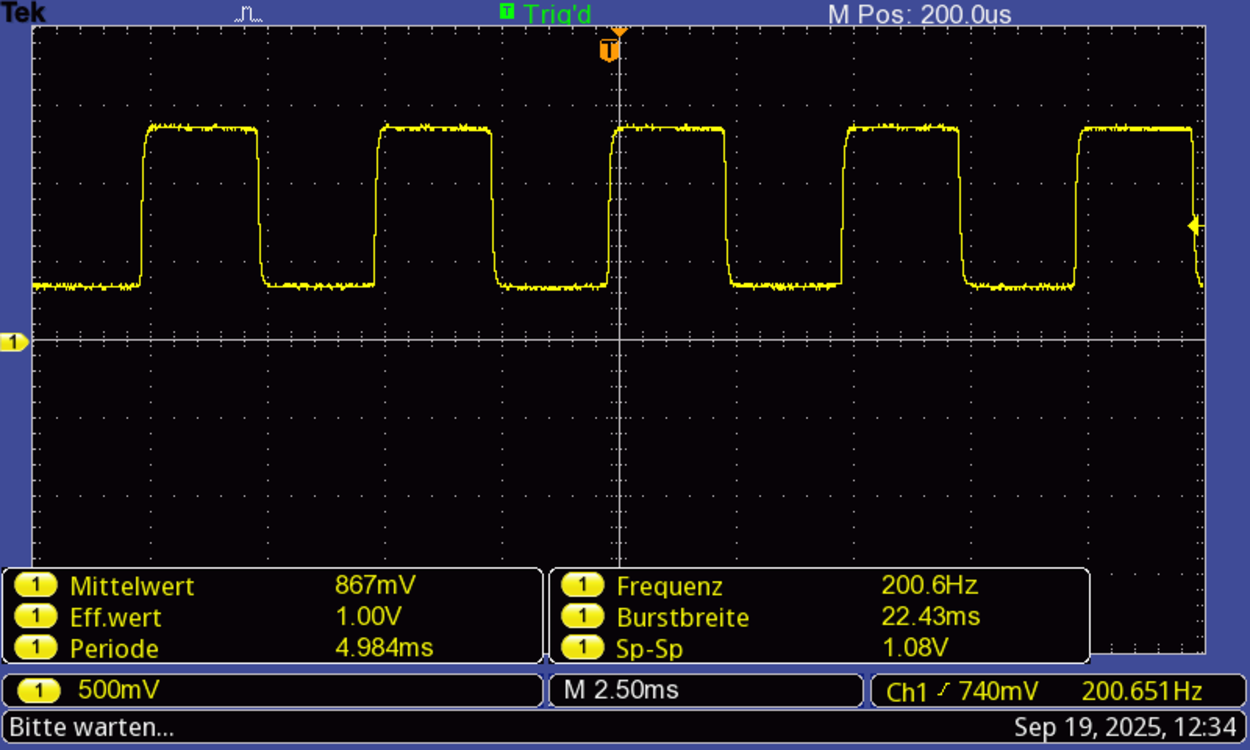
\includegraphics[width=0.45\textwidth]{img/25/Signale2/Signal1-DC.pdf}
    \caption{Signal 1 mit automatischen Messwerten und gesetzem Trigger im DC Modus.}
\end{figure}

Diese Unsicherheiten verwenden wir nun, wenn immer wir Cursor-Messungen zur Berechnung benutzen. Die automatischen Werte sollen als >>perfekt<< angenommen werden.
In den Tabellen beschreibt $T$ die Periodendauer in ms, $U_{SS}$ die Spitzen-Spitze-Spannung (also die Differenz von $U_{max}$ und $U_{min}$). $U_{max}$ und $U_{min}$ sind die lokalen\footnote{Also die auf dem Display angezeigten Extrempunkte.} Extrempunkte. $U_{G}$ ist die $DC_{offset}$-Spannung. Berechnet wird dieser über den Mittelwert im DC-Modus.

Wir schreiben daher einmal alle Informationen aus dem  \hyperref[Protokoll]{Protokoll} in zwei Tabellen, in eine für die automatisch berechneten Werte und eine für die Cursor-Messungen.

\begin{table}[h!]
    \centering
    \begin{tabular}{c | c | c | c | c }
        \toprule
        T [ms] & $U_{SS}$ [V] & $U_{G}$ [V] & $U_{max}$ [V] & $U_{min}$ [V] \\
        \hline
        4,983 & 1,06 & 0,93 & 1,50 & 0,40 \\
        \bottomrule
    \end{tabular}
    \caption{Tabelle der vom Osziloskop berechneten Werte.}
    \label{tab:sig1_auto}
\end{table}

In \hyperref[tab:sig1_auto]{Tabelle \ref*{tab:sig1_auto}} sind alle automatisch gemessenen Werte eingetragen. 

Aus der Periodendauer können wir nun die \hyperref[eq:freq]{Frequenz (\ref*{eq:freq})} berechnen:
\begin{equation}
    \boxed{
        f_{auto} = 0,202 ms^{-1} \, \hat = \, 4,95 kHz
    }.
\end{equation}

Aus den Extrema können wir $U_G$ auch noch rechnerisch über das \hyperref[eq:arithmetisches_mittel]{arithmetische Mittel \ref*{eq:arithmetisches_mittel}} bestimmen:
\begin{equation}
    U_{G,auto,r} = 0,95 V.
\end{equation}

Merkwürdig ist, dass die Werte $U_G$ und $U_{G,auto,r}$ einwenig abweichen. Dies liegt daran, dass das Signal nicht konstant war. Aus nicht bekannten Gründen sind die Werte über die Zeit angestiegen. Da wir die Werte aber nacheinander abgeschrieben haben, waren zu dem Moment die Werte schon nicht mehr stringent. Die Abweichung ist jedoch nicht besonders groß.

\begin{table}[h!]
    \centering
    \begin{tabular}{c | c | c | c }
        \toprule
        T [ms] & \textcolor{teal}{$U_{SS}$ [V]} & \textcolor{purple}{$U_{max}$ [V]} & \textcolor{purple}{$U_{min}$ [V]} \\
        \hline
        $5,00 \pm 0,16 $ & $1,064$ & $1,500$ & $0,460$ \\
        \bottomrule
    \end{tabular}
    \caption{Tabelle der mit Cursor bestimmten Werte. }
    \label{tab:sig1_cursor}
\end{table}

Wir wollen nun $U_{G}$ bestimmen. Dies ist der \hyperref[eq:arithmetisches_mittel]{Mittelwert \ref*{eq:arithmetisches_mittel}} von $U_{max}$ und $U_{min}$. 
\begin{equation}
    U_{G} = 0,980 V.
\end{equation}

Dabei entspricht $U_{G}$ gerade dem Gleichspannungsanteil.

Seinen Fehler bestimmen wir via \hyperref[eq:gauss_fehlfortpflanzung]{Gauß'scher Fehlerfortpflanzung (\ref*{eq:gauss_fehlfortpflanzung})}:
\begin{equation}
    \Delta U_{G} = \sqrt{\left(\Delta U_{min}\right)^2 + \left(\Delta U_{max}\right)^2}.
\end{equation}

Somit kommen wir auf ein Ergebnis von 
\begin{equation}
    \boxed{
        U_{G} = (980 \pm 60) \, mV
    }.
\end{equation}

Als nächstes berechnen wir die Frequenz der Cursor-Messung:
\begin{equation}
    \underline{
        f_{cursor} = 0,2 ms^{-1} \, \hat= \, 5kHz
    }.
\end{equation}

Den Fehler der Frequenz müssen wir noch bestimmen, wieder über \hyperref[eq:gauss_fehlfortpflanzung]{Gauß'scher Fehlerfortpflanzung (\ref*{eq:gauss_fehlfortpflanzung})}:
\begin{equation}
    \Delta f = \frac{\Delta T}{T^2}.
    \label{eq:f_freq}
\end{equation}

Berechenn wir diesen Fehler und tragen das Ergebnis zusammen, kommen wir zu: 
\begin{equation}
    \boxed{
        f_{cursor} = (0,200 \pm 0,006) ms^{-1}
    }.
\end{equation}
(Es wurde auf signifikante Stellen gekürzt.)


Nocheinmal die Gefragten Werte zusammengetragen:
\begin{align*}
    U_{G,auto} &= 930 mV \\
    U_{G,auto,r} &= 0,95 V \\
    U_{SS} &= 1,06 V \\
    f_{auto} &= 0,202 ms^{-1} \\
    \\
    U_{G,cursor}& = (980 \pm 60)\, mV \\
    U_{SS,cursor} &= (1\,064 \pm 15)\, mV \\
    U_{SS,cursor,r} &= (1\,040 \pm 60)\, mV \\
    f_{cursor} &= (0,200 \pm 0,006)\, ms^{-1}
\end{align*}

Der Wert $U_{SS,cursor,r}$ ist dabei der nochmal neu gerechtete Wert, aus dem Maximum und dem Minimum. 

Wir berechnen nun noch, wie signifikant die Werte des Cursors sind, indem wir die autoamtisch berechneten als Referent nehmen. Wir nuzen \hyperref[eq:signifikante_abweichung]{Gleichung \ref*{eq:signifikante_abweichung}} der Fehlerrechnung:
Wir beginnen mit der Offset-Spannung $U_G$:
\begin{equation}
    \frac{\left| U_{G,auto} - U_{G,cursor} \right|}{\Delta U_{G,cursor}} = 0,83\sigma.
\end{equation}

Für die Spitzen-Spitzen-Spannung:
\begin{equation}
    \frac{\left| U_{SS,auto} - U_{SS,cursor} \right|}{\Delta U_{SS,cursor}} = 0,26\sigma.
\end{equation}

Und zuletzt für die Frequenz:
\begin{equation}
    \frac{\left| f_{auto} - f_{cursor} \right|}{\Delta f_{cursor}} = 0,33\sigma.
\end{equation}


% \begin{figure} [h!]
%     \centering
%         
\includegraphics[width=0.35\textwidth]{img/25/memes/kommunismus.pdf}
%     \caption{Meme nach Signal 1}
% \end{figure}


% ------------------- Signal 2 -------------------

\subsection*{Signal 2}
\begin{figure} [h!]
    \centering
        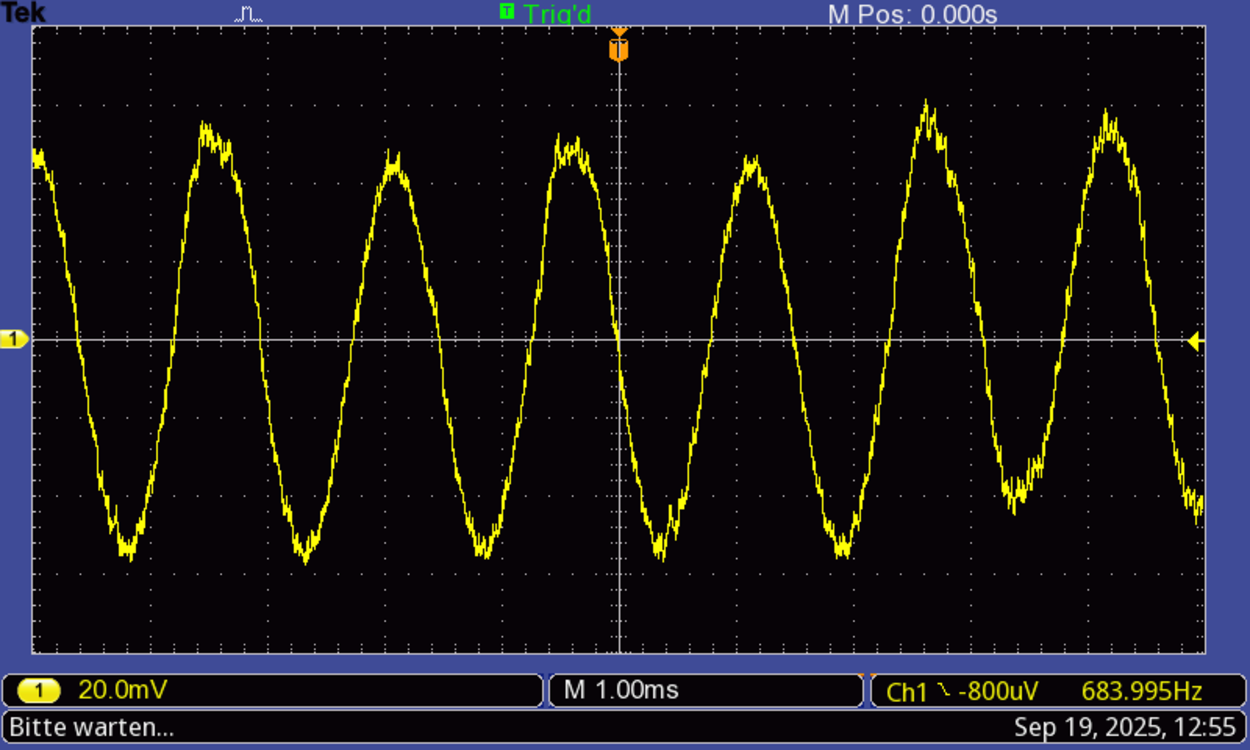
\includegraphics[width=0.45\textwidth]{img/25/Signale2/Signal2-Clean.pdf}
    \caption{Signal 2 mit gesetzem Trigger.}
\end{figure}

Wir schauen uns nun das zweite Signal an, dessen Punkte wir gemessen haben. Die Tabellen sind hier wie bei Signal 1 Aufgebaut.

\begin{table}[h!]
    \centering
    \begin{tabular}{c | c | c | c | c }
        \toprule
        T & $U_{SS}$ [V] & $U_{G}$ [V] & $U_{max}$ [V] & $U_{min}$ [V] \\
        \hline
        --- & 0,104 & 1,61 & -1,56 & -1,67 \\
        \bottomrule
    \end{tabular}
    \caption{Tabelle der vom Osziloskop berechneten Werte des zweiten Signals.}
    \label{tab:sig2_auto}
\end{table}

Die Periodendauer konnte automatisch nicht gemessen werden. Dies lag an dem stark rauschendem (beziehungsweise nicht konstanen) Signal. Auch wenn man es pausiert, kann keine automatische Periodenmessung stattfinden. Als logische Konsequenz kann hier keine Frequenz bestimmt werden.

Neben den automatisch berechneten Werten für $U_{SS}$ und $U_G$ wollen wir die Rechnung über die $U_{max}$ und die $U_{min}$ nochmal überprüfen:
\begin{equation}
    U_{SS,r} = 0,11 V,
\end{equation}
\begin{equation}
    U_{G,r} = 1,615 V.
\end{equation}

Es sind leichte Abweichungen zu erkennen, aber grundsätzlich sind die Werte stringent. Die Abweichungen kommen wie bei Signal 1 daher, dass die Signale nicht kontinuirlich sind, sonder Schwankungen unterliegen. 

Für die Cursor-Messung müssen wir zunächst wieder die Fehler bestimmen. Wir haben dieses mal für die AC-Spannung ein Step-Grid von $20mv \times 1,00ms$. Für die DC-Spannung $50mv \times 1,00ms$. Wir greifen wieder auf die \hyperref[tab:all_fehler]{Tabelle \ref*{tab:all_fehler}} zurück und kommen somit auf Ungenauigkeiten von:
\begin{align}
    \Delta t &= 0,006 ms \\
    \textcolor{teal}{\Delta U_{AC}} &=1,5 mV \\
    \textcolor{purple}{\Delta U_{DC}} &= 4,0 mV
\end{align}

Wir tragen nun die Werte der Messungen in die Tabelle ein:
\begin{table}[h!]
    \centering
    \begin{tabular}{c | c | c | c }
        \toprule
        T [ms] & \textcolor{teal}{$U_{SS}$ [mV]} & \textcolor{purple}{$U_{max}$ [mV]} & \textcolor{purple}{$U_{min}$ [mV]} \\
        \hline
        $1,560$ & $125,6$ & $68,8$ & $56,8$ \\
        \bottomrule
    \end{tabular}
    \caption{Tabelle der mit Cursor bestimmten Werte. }
    \label{tab:sig2_cursor}
\end{table}

Wir berechen die \hyperref[eq:freq]{Frequenzen (\ref*{eq:freq})} Cursor- Messung:
\begin{equation}
    f_{cursor} = 0,641 ms^{-1}.
\end{equation}

Sein Fehler wird Analog zu \hyperref[eq:f_freq]{Gleichung \ref*{eq:f_freq}} berechnet. Wir kommen also auf ein Ergebnis von
\begin{equation}
\boxed{
    f = (0,6410 \pm 0,0025) \, ms^{-1}
}.
\end{equation}

Als nächstes wollen wir $U_G$ aus der Cursor-Messung bestimmen. Diese ist wieder Analog zum ersten Signal. 
Unser $U_{G,cursor}$ ist somit:
\begin{equation}
    U_{G,cursor} = 62,8 mV,
\end{equation}
mit einer Ungenauigkeit von
\begin{equation}
    \Delta U_{G,cursor} = 5,657 mV.
\end{equation}

Als Ergebnis also:
\begin{equation}
\boxed{
    U_{G,cursor} = (63 \pm 6) \, mV
}.
\end{equation}

Recht offensichtlich ist der gemessene Wert der $U_{SS}$-Spannung nicht richtig. Wir würden eigentlich erwarten:
\begin{equation}
    U_{SS,r} = 12 mV
\end{equation}

Der oben angegebene Wert ist scheinbar einfach die Summe der Extrema. Diese Berechnung ist flasch. Wir haben diesen Wert hier also offensichtlich nicht gemessen, sondern falsch berechnet. Von nun an ist $U_{SS,r}$ der richtige Wert.
Wir müssen seine Ungenauigkeit noch bstimmen. Diese ist jedoch einfach identisch zur $U_G$-ungenauigkeit. Unser Ergebnis ist somit:
\begin{equation}
    \boxed{
        U_{SS,cursor} = (12 \pm 6) mV
    }.
\end{equation}

Zum Schluss des zweiten Signals noch die Abweichungen:

Offset-Spannung:
\begin{equation}
    \frac{\left| U_{G,auto,2} - U_{G,cursor,2} \right|}{\sqrt{(\Delta U_{G,cursor,2})^2}} = 257,84\sigma
\end{equation}

Spitzen-Spitzen-Spannung:
\begin{equation}
    \frac{\left| U_{SS,auto,2} - U_{SS,cursor,2} \right|}{\sqrt{(\Delta U_{SS,cursor,2})^2}} = 15,33\sigma
\end{equation}

\newpage
\onecolumn
\twocolumn

% ------------------- Signal 3 -------------------
\subsection*{Signal 3}
\begin{figure} [h!]
    \centering
        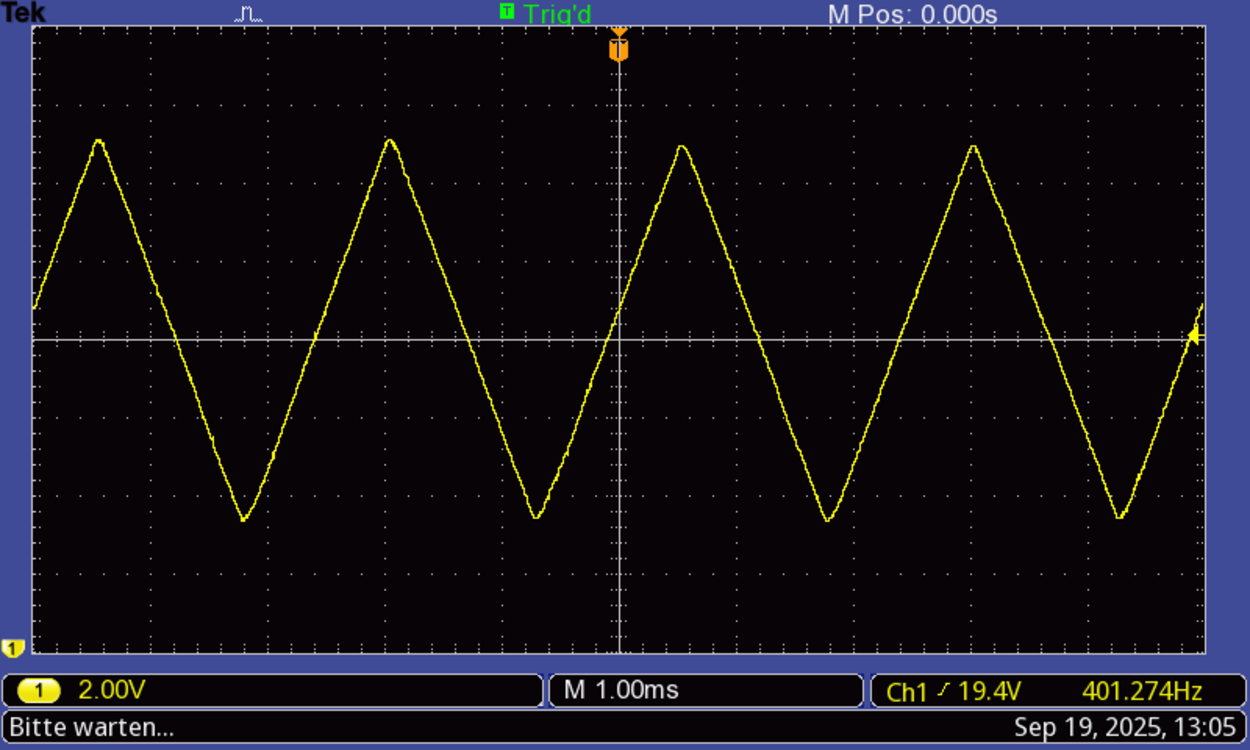
\includegraphics[width=0.45\textwidth]{img/25/Signale2/Signal3.pdf}
    \caption{Signal 3}
\end{figure}

Das gemessene Signal 3 weist eine periodische Zickzackstruktur auf. Es besteht aus linearen Anstiegs- und Abfallflanken mit annähernd konstanter Steigung. Die Wiederholung der linearen Strecken kennzeichnet ein gleichmäßiges Muster mit konstanter Periodendauer. Die Signalform entspricht typischen Dreieckssignal.

% ------------------- Signal 4 -------------------
\subsection*{Signal 4}
\begin{figure} [h!]
    \centering
        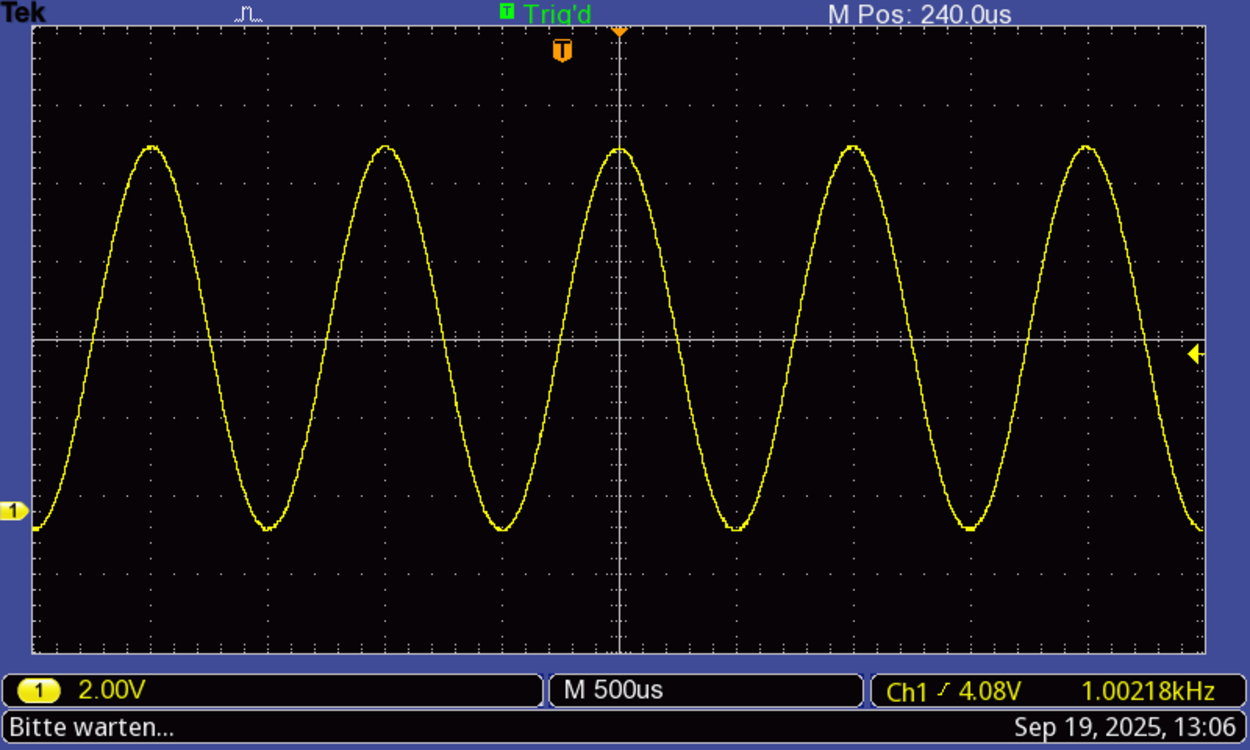
\includegraphics[width=0.45\textwidth]{img/25/Signale2/Signal4.pdf}
    \caption{Signal 4}
\end{figure}

Das gemessene Signal 4 zeigt einen periodischen Sinusverlauf. Es weist eine gleichmäßige, harmonische Schwingung mit kontinuierlichem Übergang zwischen Maxima und Minima auf.

\newpage

% ------------------- Signal 5 -------------------
\subsection*{Signal 5}

Für Signal 5 ist die Halbwertszeit zu bestimmen, also jene Zeit, bei der die Spannung um die Hälfte abgefallen ist.
Gemessen haben wir mit einer Divgröße von $500mV \times 2,5ms$ berechnet. Das Spannungsplatau lag bei $1V$. Wir haben also geschaut, wie groß die x-Achsen-Differenz vom Punkt, wo die Spannung abfällt, bis zu dem Punkt, an dem sie $500mV$ beträgt.

\begin{figure} [h!]
    \centering
        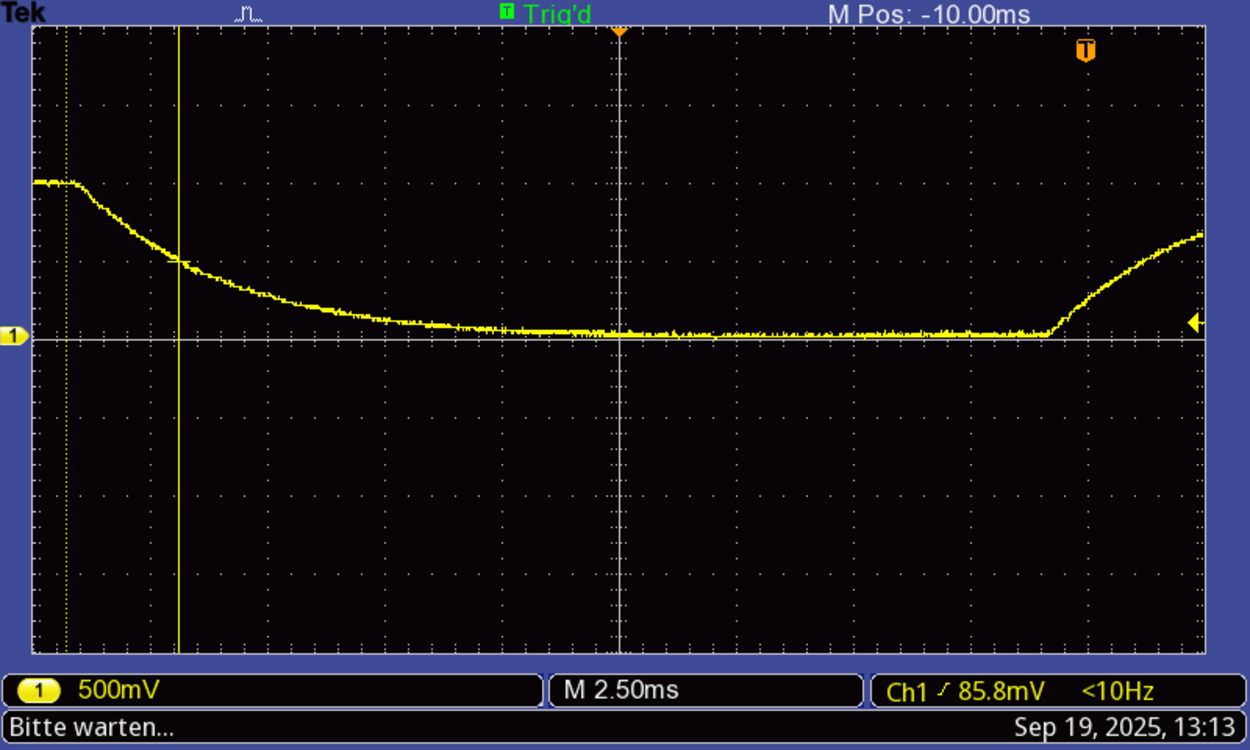
\includegraphics[width=0.45\textwidth]{img/25/Signale2/Signal5-Clean.pdf}
    \caption{Signal 5 nah rangezoomed um den Abfall klar zu erkennen.}
\end{figure}

Die Halbwertszeit liegt dabei bei 
\begin{equation}
    2,40 ms
\end{equation}.

Wir haben eine Auflösung von 2,5ms, wir haben also einen Zeitfehler von:
\begin{equation}
    0,15 ms
\end{equation}

Wir tragen das gesamte zu einem Ergebnis zusammen:
\begin{equation}
\boxed{
    t_H = (2,40 \pm 0,15)\, ms
}
\end{equation}


Außerdem sind hier nochmal die beiden Grafiken, die zum Vergleich der AC und der DC-Spannung dienen. Abbildung \ref{fig:sig5-ac} zeigt die AC-Spannung, Abbildung \ref{fig:sig5-dc} die DC-Spannung.
\onecolumn
\begin{figure} [h!]
    \centering
        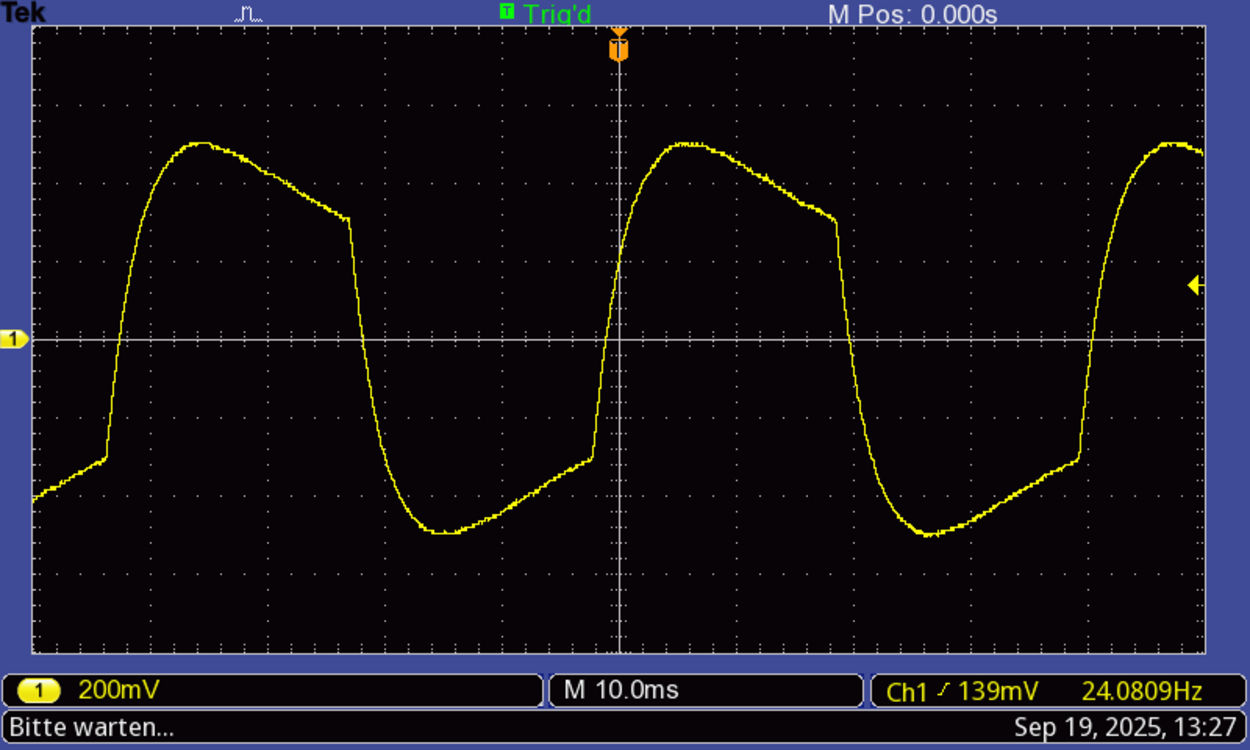
\includegraphics[width=0.8\textwidth]{img/25/Signale2/Signal5-AC.pdf}
    \caption{Signal 5-AC modus}
    \label{fig:sig5-ac}
\end{figure}

\begin{figure} [h!]
    \centering
        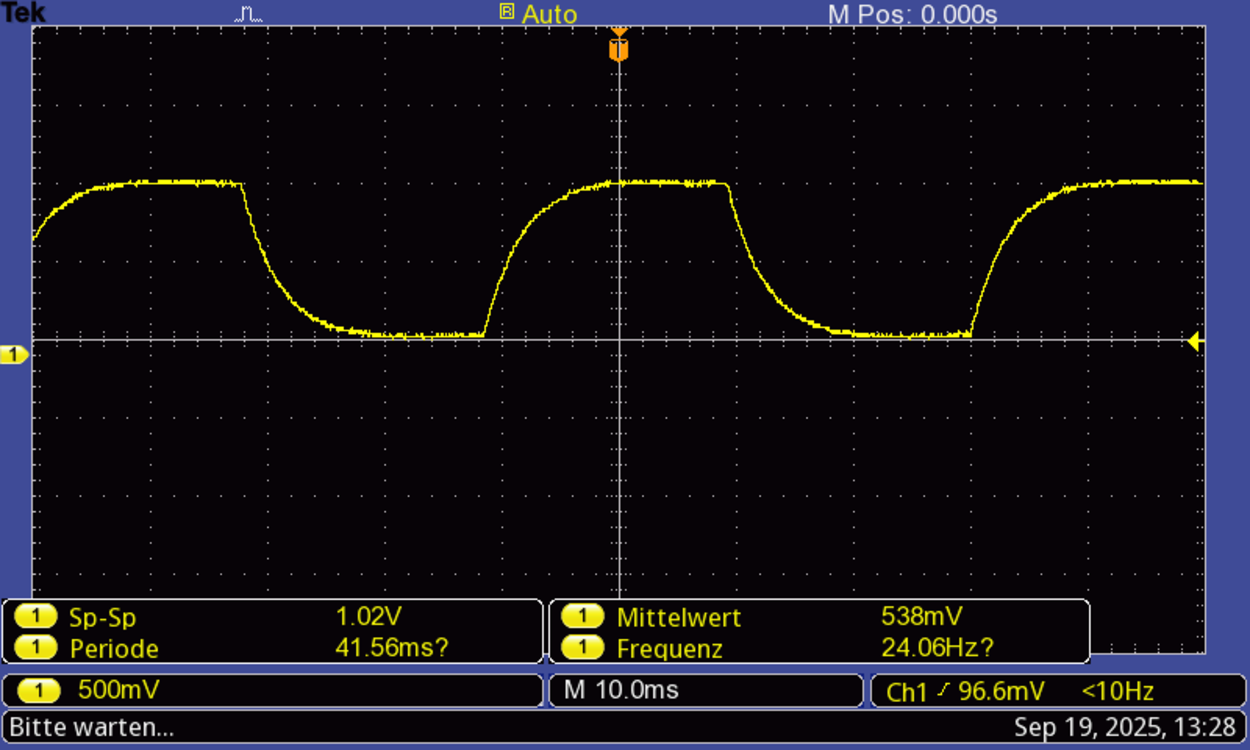
\includegraphics[width=0.8\textwidth]{img/25/Signale2/Signal5-DC.pdf}
    \caption{Signal 5-DC Modus}
    \label{fig:sig5-dc}
\end{figure}
\twocolumn

\newpage
\onecolumn
\twocolumn

% ------------------- Signal 6 -------------------
\subsection*{Signal 6}
\begin{figure} [h!]
    \centering
        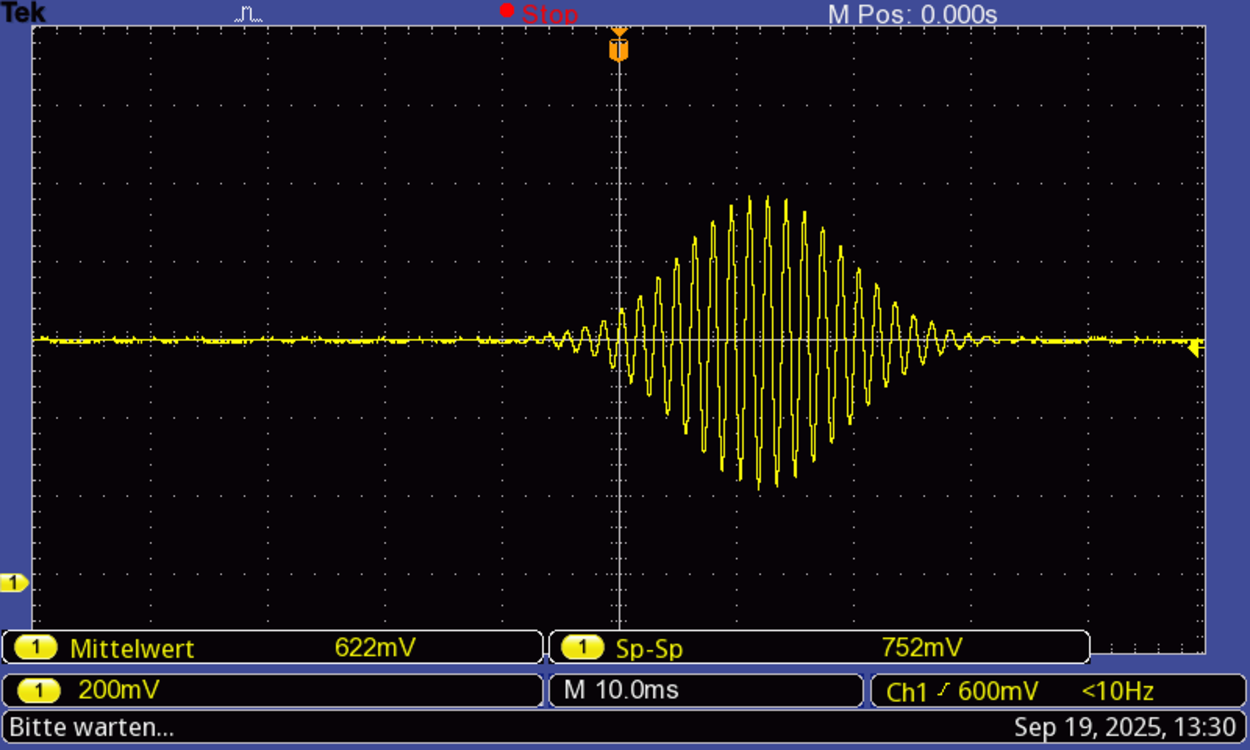
\includegraphics[width=0.45\textwidth]{img/25/Signale2/Signal6.pdf}
    \caption{Signal 6}
\end{figure}

Das hier gezeigte Signal 6 ist eine kurzer Puls. Dieser ist eine Sinuskurve, mit nicht konstanter Amplitude.

% ------------------- Signal 7 -------------------
\subsection*{Signal 7}
\begin{figure} [h!]
    \centering
        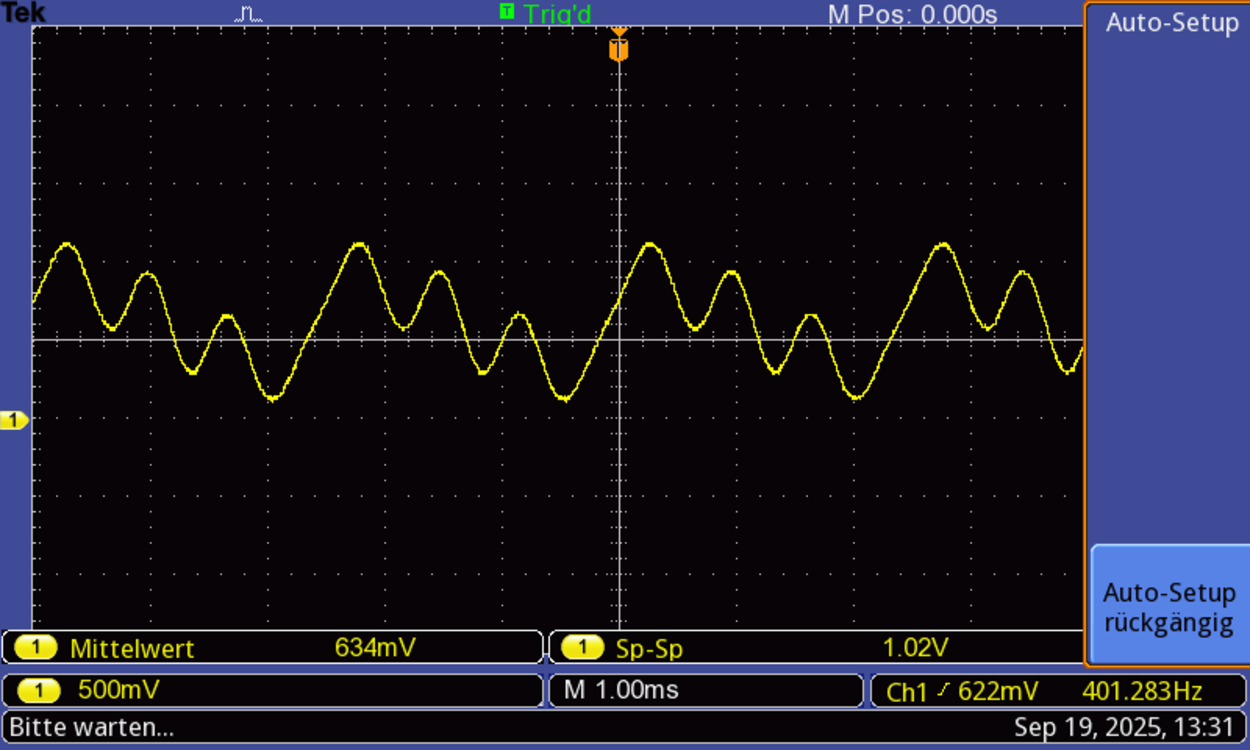
\includegraphics[width=0.45\textwidth]{img/25/Signale2/Signal7.pdf}
    \caption{Signal 7}
\end{figure}

Das Signal 7 Zeigt eine periodische Sinuskurve. Diese ist jedoch nicht harmonisch, sie scheint eine Überlagerung verschiedener Sinuskurven zu sein.

\newpage

% ------------------- Signal 8 -------------------
\subsection*{Signal 8}
\begin{figure} [h!]
    \centering
        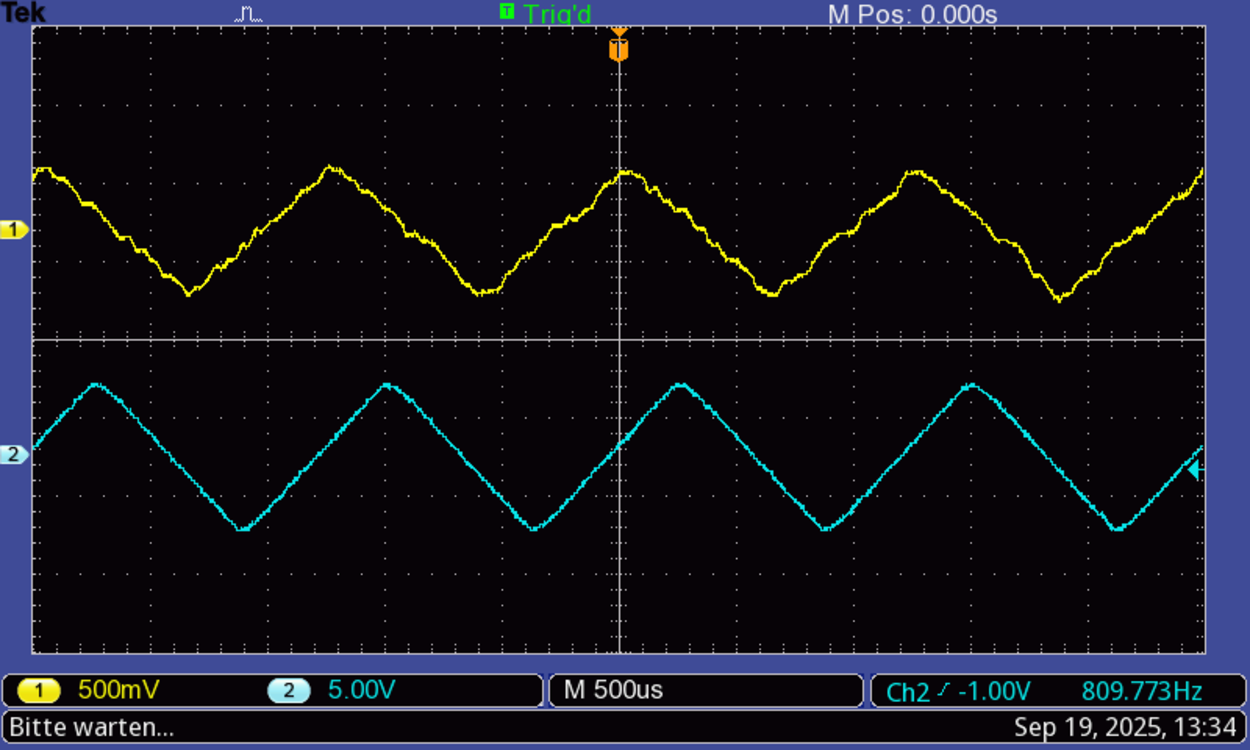
\includegraphics[width=0.45\textwidth]{img/25/Signale2/Signale8-deutlich-getrennt.pdf}
    \caption{Signal 8 mit verschobenen Nullpunkten und verschiedenen Amplituden.}
\end{figure}

\begin{figure} [h!]
    \centering
        \includegraphics[width=0.45\textwidth]{img/25/Signale2/Signale8-Überlagerung.pdf}
    \caption{Signal 8 mit gleichem Nullpunkt, aber verschiedenen Amplituden.}
\end{figure}

Das Signal 8 zeigt zwei Zick-Zack-Signale, welche zum einen eine leichte Phasenverschiebung haben (geschätzt ca. 350$\mu$s). Die Amplitude des Signals aus Kanal 2 (blau) ist etwas über 10-Mal größer (ca. 400mV vs. 4\,800 mV).

\newpage 

% ------------------- Signal 9 -------------------
\subsection*{Signal 9}

Für Signal 9 sind wieder Messungen betrieben wurden. D
\begin{figure} [h!]
    \centering
        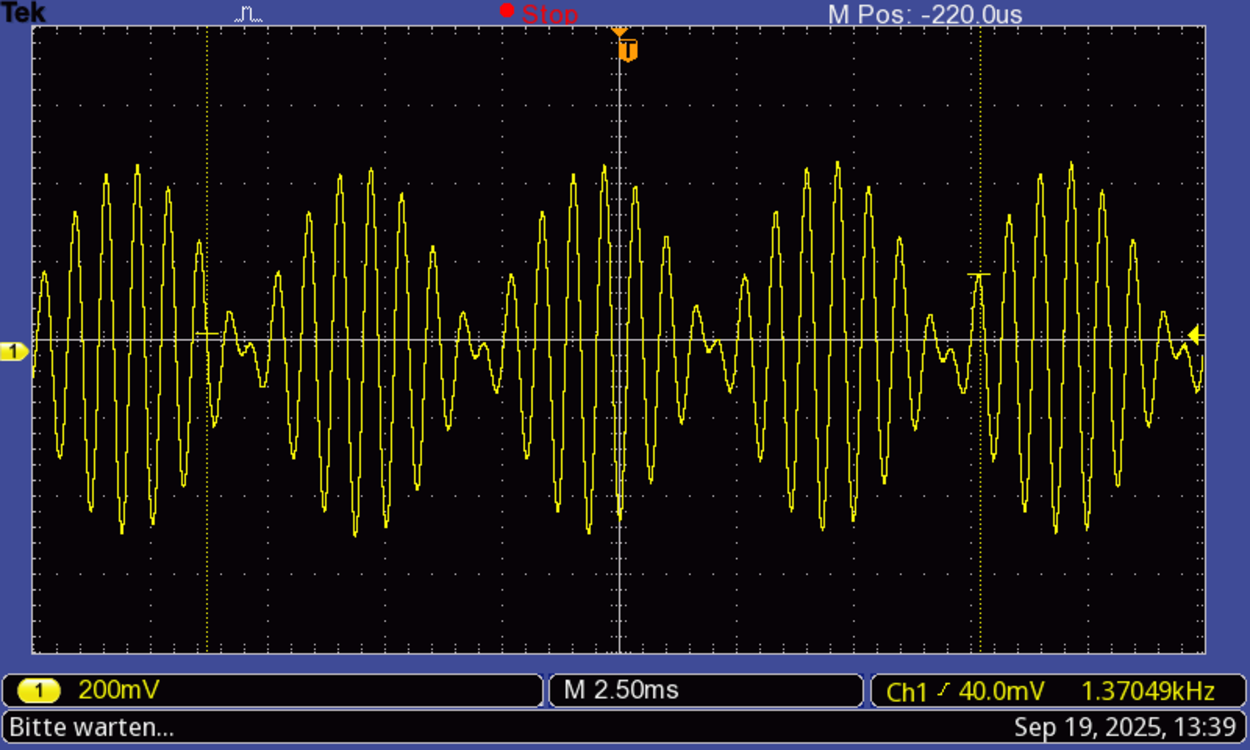
\includegraphics[width=0.45\textwidth]{img/25/Signale2/Signal9-Gesamt.pdf}
    \caption{Signal 9. Man sieht die Pahsen und die Gruppen sehr gut}
    \label{fig:s9_ges}
\end{figure}

\hyperref[fig:s9_ges]{Abbildung \ref*{fig:s9_ges}} zeigt das gemessene Signal mit einer recht geringen Zeitstauchung. Man sieht hier Gruppen und Phasen des Signals. Die \hyperref[fig:s9_phahue]{Abbildung \ref*{fig:s9_phahue}} zeigt dabei die Einhüllung einer Phase.

\begin{figure} [h!]
    \centering
        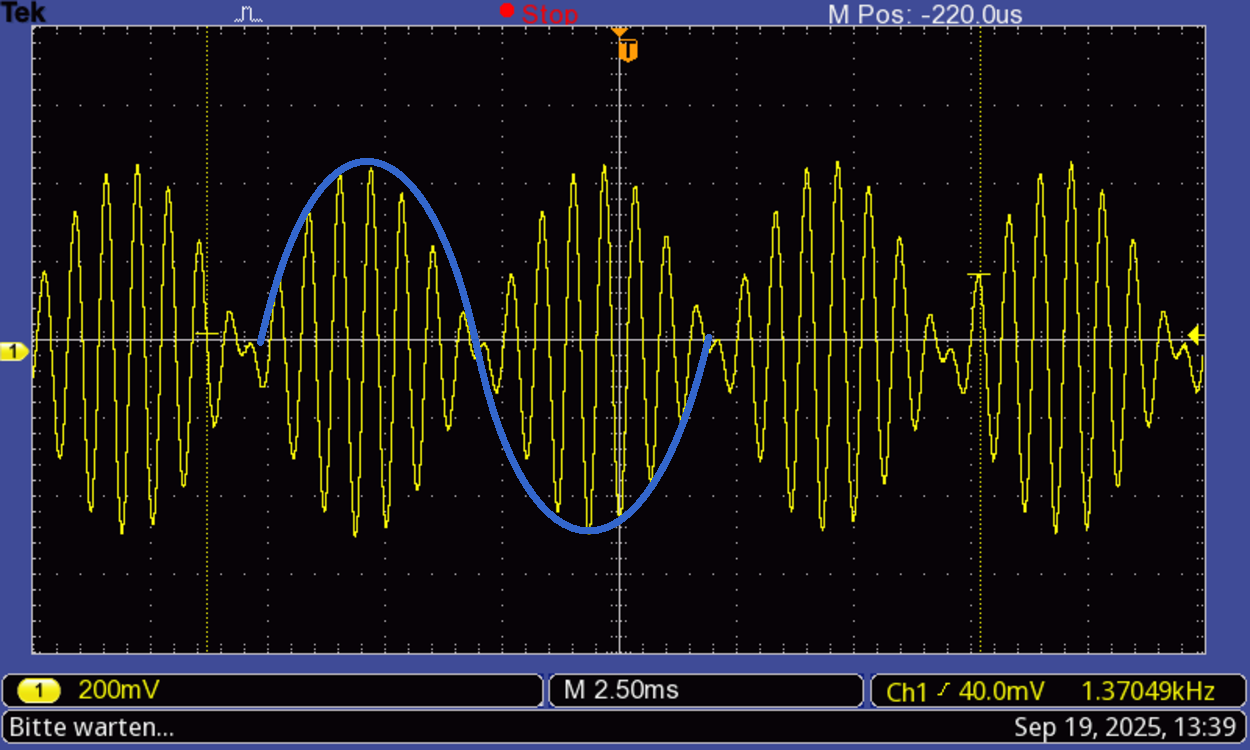
\includegraphics[width=0.45\textwidth]{img/25/Signale2/Signal9-Sin-eingezeichnet.pdf}
    \caption{Signal 9 mit eingezeichneter Phasenhülle.}
    \label{fig:s9_phahue}
\end{figure}

Verfeinert man die Zeitskala, so lässt sich auch eine einzelne Gruppe begutachten, wi in \hyperref[fig:s9_einzeln]{Abbildung \ref*{fig:s9_einzeln}}.

\begin{figure} [h!]
    \centering
        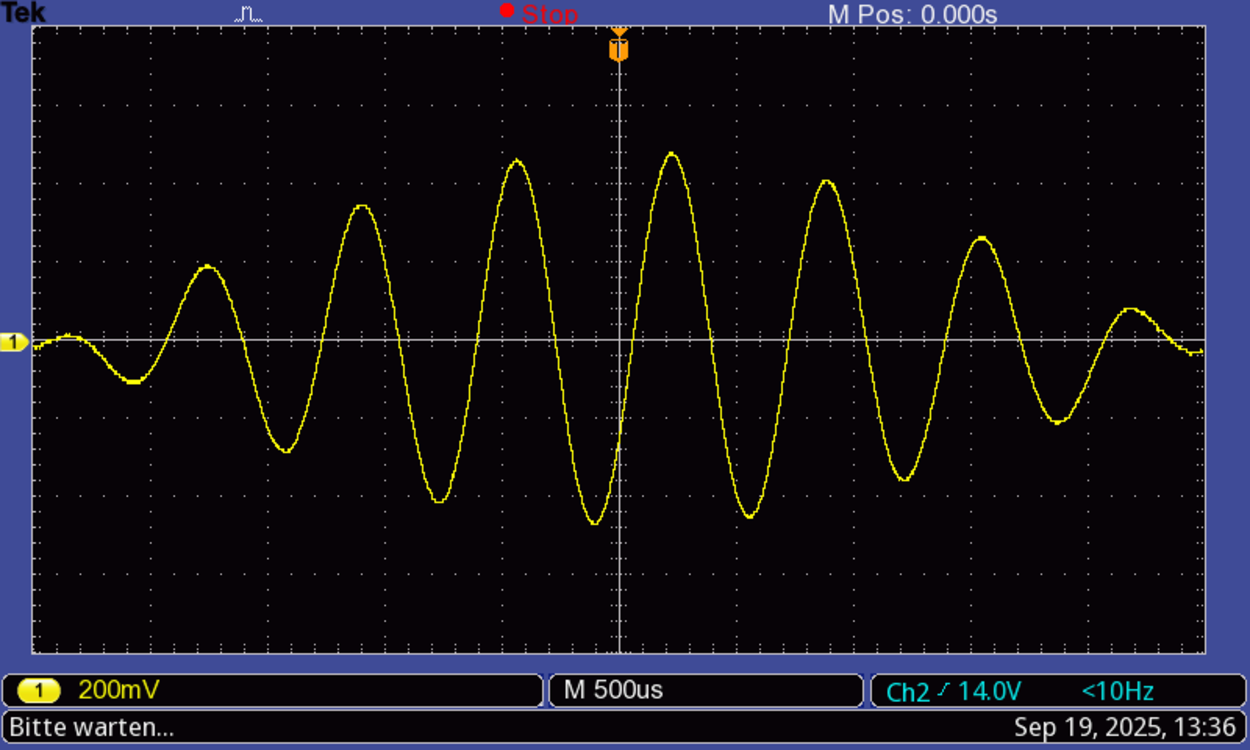
\includegraphics[width=0.45\textwidth]{img/25/Signale2/Signal9-einzeln.pdf}
    \caption{Signal 9, einzelne Gruppe.}
    \label{fig:s9_einzeln}
\end{figure}

Damit so ein Signal möglich ist, müssen mindestens zwei Signale überlagern und sich destruktiv und konstruktiv beweinflussen. Aus der Aufgabe ist klar, dass es hier zwei Sinussignale mit konstanter Frequenz sind. Diese zwei Eigenfrequenzen wollen wir bestimmen und nutzen dafür den FFT-Modus (Fast-Fouriertransformation).
Das Resultat ist in \hyperref[fig:s9_fft]{Abbildung \ref*{fig:s9_fft}} gezeigt. 
Hier müssen beide Berge mit den Cursorn vermessen werden.

\begin{figure} [h!]
    \centering
        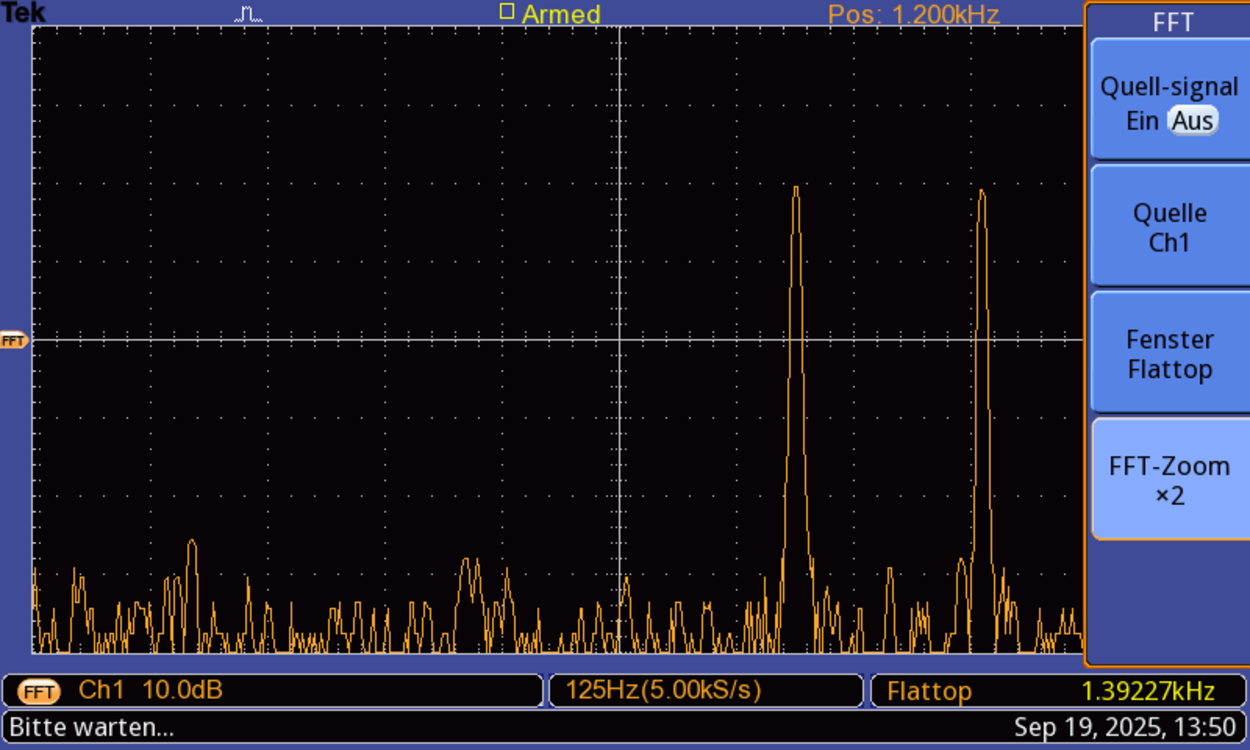
\includegraphics[width=0.45\textwidth]{img/25/Signale2/Sig9-FFT.pdf}
    \caption{Signal 9 alt FFT-Signal.}
    \label{fig:s9_fft}
\end{figure}

Wir entnehmen dem \hyperref[Protokoll]{Protokoll} die Werte der Tabelle 3. Gemessen haben wir in einem $200mV \times 500 \mu s$ Div-Grid, wie in \hyperref[fig:s9_einzeln]{Abbildung \ref*{fig:s9_einzeln}}.
Dabei haben wir die Dauer von 5 Perioden vermessen. Unsere 500$\mu$s führen zu einer Zeitungenauigkeit von $31,5 \mu$s. Unser gemessenes Ergebnis ist also:
\begin{equation}
\underline{
    T_5 = (3,30 \pm 0,03) \, ms
}
\end{equation}

Wir devidieren das Ergebnis mit 5 und kommen somit auf eine Periodendauer von 
\begin{equation}
\boxed{
    T = (0,660 \pm 0,006) \, ms
}.
\end{equation}

Zur Berechnung der Frequenz müssen wir lediglich den Kerwert der Periodendauer nehmen. Der Fehler der Frequenz berechnet sich analog zu \hyperref[eq:f_freq]{Gleichung \ref*{eq:f_freq}}. Wir kommen somit auf eine Frequenz von
\begin{equation}
\boxed{
    f_1 = (1,515 \pm 0,014) \, ms^{-1}
}.
\end{equation}

$f_1$ ist die Schwingfrequenz. Als nächstes wollen wir die Schwbungsfrequenz $f_2$ bestimmen. Dies entspricht der Periodendauer der Einhüllenden wie in \hyperref[fig:s9_phahue]{Abbildung \ref*{fig:s9_phahue}} gezeigt. Das Grid ist $200mV \times 2,5ms$ Groß.
Der zeitzliche Fehler beträgt hier also $\Delta t = 0,1575ms$. Leider ist uns hier abermals ein Fehler unterlaufen, wir haben hier direkt eine Frequenz berechnet, so können wir jedoch die Ungenauigkeit nicht bestimmen. Es ist etwas kompliziert jetzt an die richtig Periodendauer der Schwebung zu kommen, aber nicht unmöglich. Zum lösen dieses Problemes habe ich das Bild in ein Grafik-Programm geladen und die Breite des gesamten Containers berechnet und die Breite der Periode. Dies ist der \hyperref[fig:s9_Pschweb]{Abbildung \ref*{fig:s9_Pschweb}} zuentnehmen. Dabei wurde darauf geachtet, die Striche, die die Periode eingrenzen, um $\frac{1}{250}$ Steps zu bewegen. Die Striche sind für das Bild breiter geamcht wurden, zur Messung waren diese auf 0,001mm gestellt, diese waren jedoch nicht auf einem Bild zu erkennen. Die Messung fand dennoch mit diesen Statt, dies sind auch die angezeigten Werte.

\begin{figure} [h!]
    \centering
        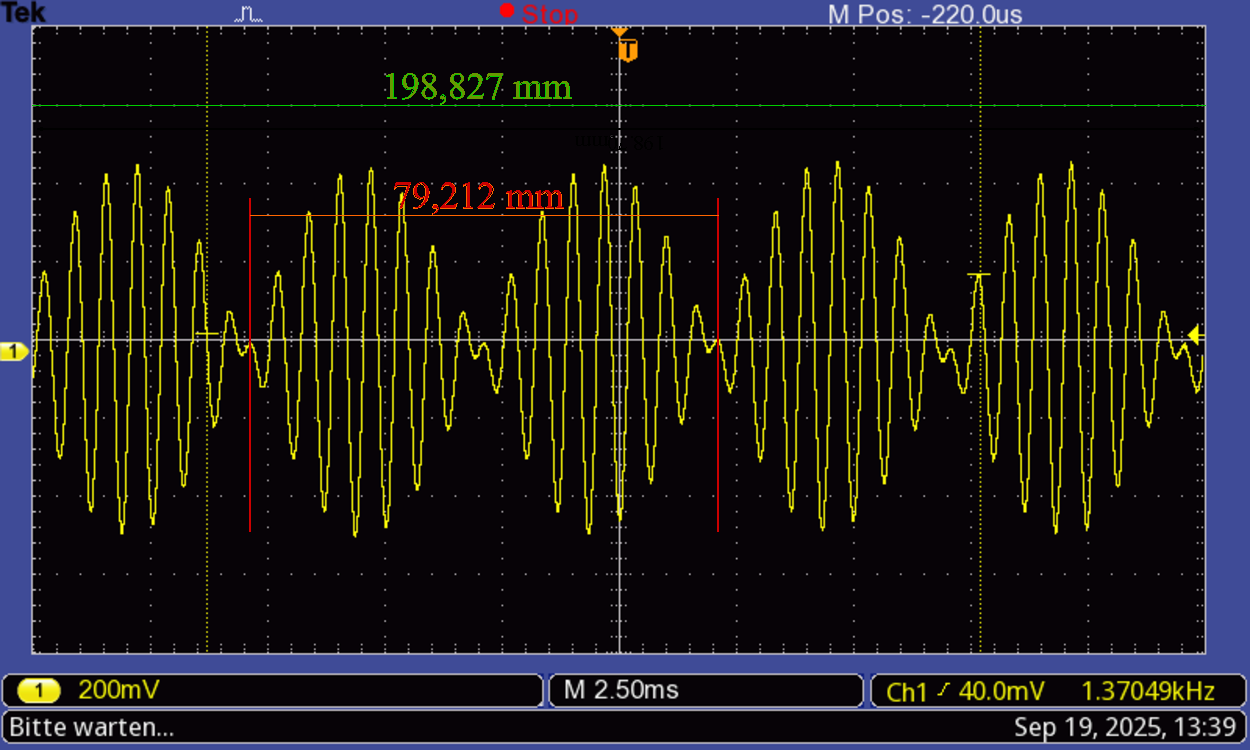
\includegraphics[width=0.45\textwidth]{img/25/Signale2/Sig9-PeriodeSchwebung.pdf}
    \caption{Signal 9 Periode mit eingezeichneten Größen.}
    \label{fig:s9_Pschweb}
\end{figure}

Wir haben eine Breite von 10 Divisions, mit je einer Breite von 2,5ms, somit ist die Gesamtbreite 25ms. Wir können nun das Verhältnis der beiden Breiten berechnen
\begin{equation}
    \frac{79,212 mm}{198,827 mm} = 0,398
\end{equation}

und dieses Ergebnis mit der Gesamtbreite multiplizieren
\begin{equation}
    0,398 \cdot 25ms = 9,95ms.
\end{equation}

Wir kommen somit auf eine Periodendauer der Schwebung von:
\begin{equation}
\boxed{
    T_{2} = (9,95 \pm 0,16) \, ms
}.
\end{equation}

Wir berechnen erneut die Frequenz und kommen dabei auf:
\begin{equation}
\boxed{
    f_2 = (0,101 \pm 0,016) \, ms^{-1}
}.
\end{equation}

Im nächsten schritt wollen wir die spezifischen Eigenfrequenzen der beiden Sinus-Funktionen $f_{i}$ und $f_{ii}$ bestimmen. 
Dafür sind wir in den FFT-Modus gewechselt und haben die beiden Peaks des Signals mit dem Cursor vermessen. Die Messwerte sind folgende:
\begin{align}
    f_{i} = 1390 Hz \\
    f_{ii} = 1590 Hz.
\end{align}

Den Fehler hier abzuschätzen war nicht besonders einfach\footnote{Die folgende Abschätzung war nicht wirklich nötig, ein Div sind $125Hz \cdot 2$, da wir einen doppelten Zoom haben. Es wird nochmal die tatsächliche Skala verwendet.}. Aber mit einem analogen Verfahren wie zur Bestimmung der Periode lässt sich auch im FFT-Modus arbeiten. 
Wir bestimmen die Höhe eines Divs und die Höhe der beiden Peaks. Diese sind der \hyperref[fig:s9_fft_ung]{Abbildung \ref*{fig:s9_fft_ung}} zu entnehmen.

\begin{figure} [h!]
    \centering
        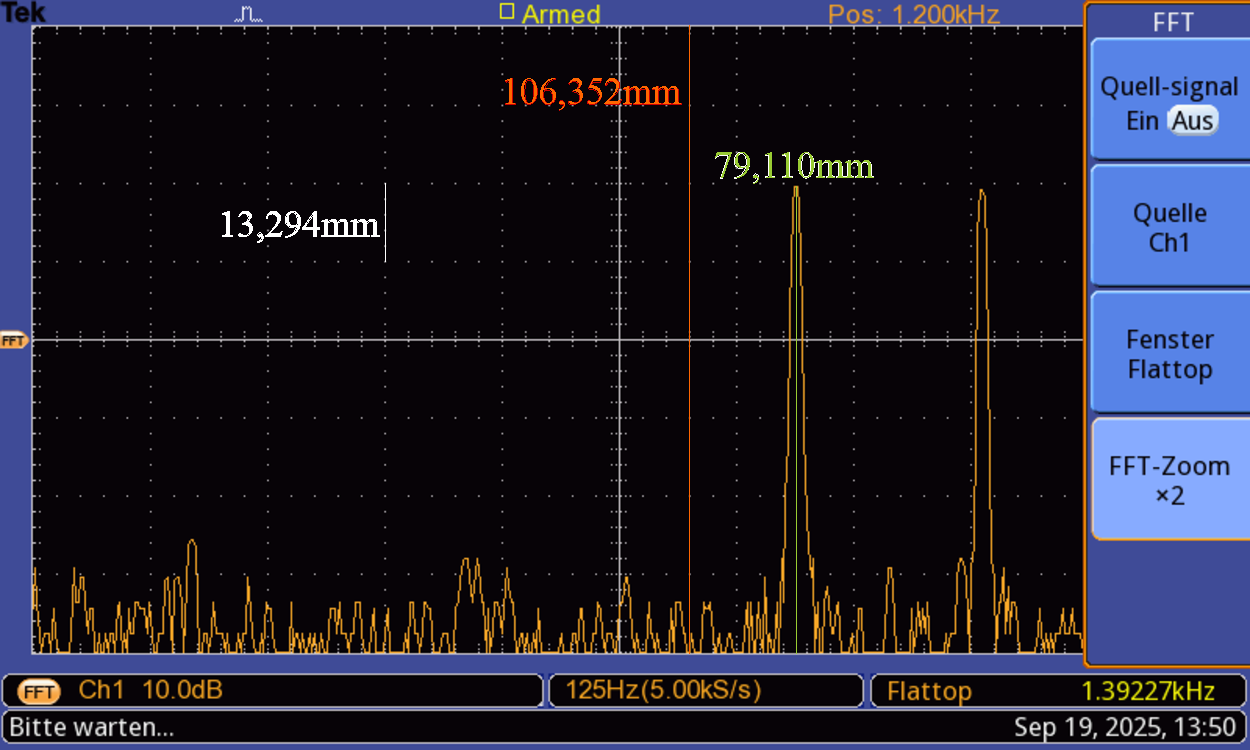
\includegraphics[width=0.45\textwidth]{img/25/Signale2/Sig9-FFT-ungenauigkeiten.pdf}
    \caption{Signal 9 FFT-Signal mit eingezeicheten Größen.}
    \label{fig:s9_fft_ung}
\end{figure}

Ein Div sind also 13,294mm. das Signal $f_{ii} = 1590 Hz \hat = 79,110mm$. Wir brechnen zu nächst, wie viele DIVs der Peak hoch ist:
\begin{equation}
    h_{ii} = \frac{79,110mm}{13,294mm} = 5,951 DIVs.
\end{equation}

Damit können wir nun den Wert eines DIVs bestimmen:
\begin{equation}
    \frac{1590}{5,951} = 267,182 \frac{Hz}{Div}.
\end{equation}

Wir haben wieder die 8 DIVs, mit á 25 Steps, somit kommen wir auf eine Step-Ungenauigkeit von:
\begin{equation}
    \Delta f = \frac{1}{200} Div \cdot 267,182 \frac{Hz}{Div} = 1,33591 Hz.
\end{equation}

Somit sind unsere Ergebnisse einmal für die $f_{i}$
\begin{equation}
    \boxed{
        f_{i} = (1390,0 \pm 1,3) Hz
    }
\end{equation}
und für $f_{ii}$
\begin{equation}
    \boxed{
        f_{ii} = (1590,0 \pm 1,3) Hz
    }
\end{equation}

\subsection*{Korrektur mit 250Hz/Div}
\begin{equation}
    \Delta f = \frac{1}{200} Div \cdot 250 \frac{Hz}{Div} = 1,25 Hz.
\end{equation}

Somit sind unsere Ergebnisse einmal für die $f_{i}$
\begin{equation}
    \boxed{
        f_{i} = (1390,00 \pm 1,25) Hz
    }
\end{equation}
und für $f_{ii}$
\begin{equation}
    \boxed{
        f_{ii} = (1590,00 \pm 1,25) Hz
    }
\end{equation}
\newpage
\onecolumn
\twocolumn


% ////////////  Aufgaben Wechsel ////////////
\section{Aufgabe 3: Pulsweitenmodulation}
Nun werden Signale eines Pulsweitenmodulators analysiert. Wir haben an einem Drehregler zwei verschiedene Signale eingestellt. Das Ziel war es, möglichst nah an 50\% und 25\% Pulsdauer-zu-Periodendauer zu kommen.

\begin{figure} [h!]
    \centering
        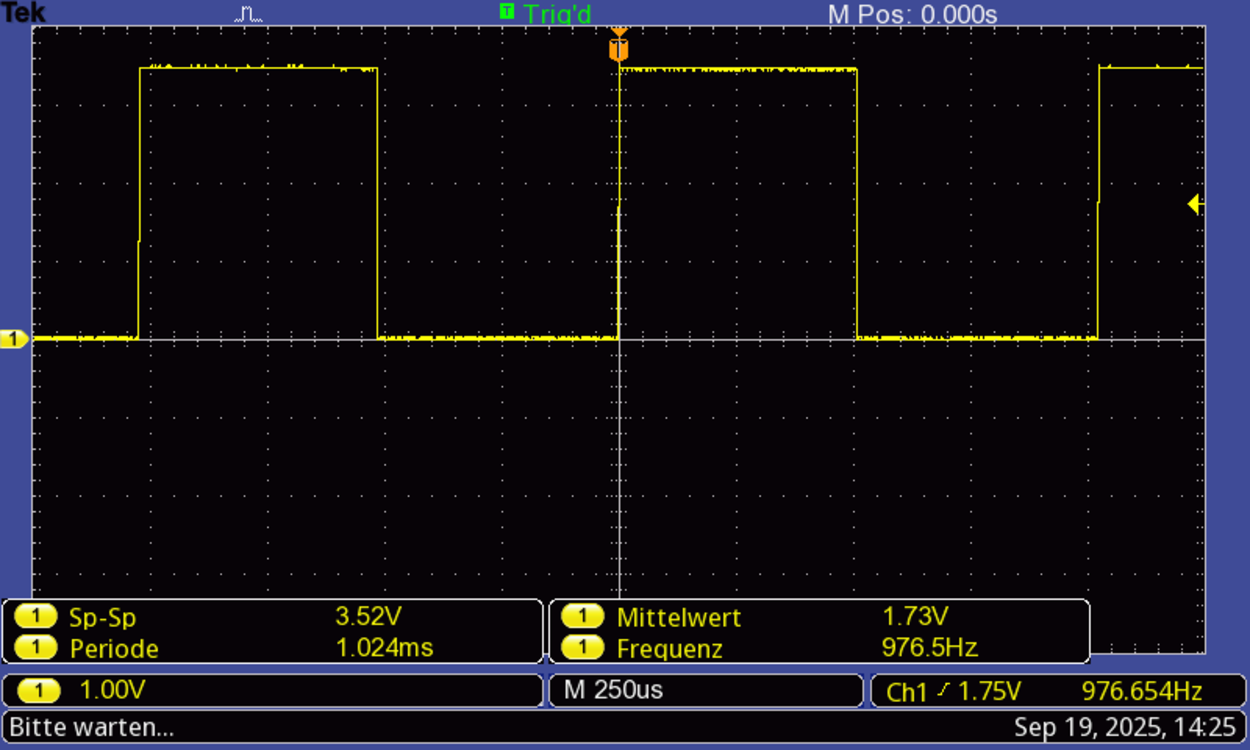
\includegraphics[width=0.45\textwidth]{img/25/Puls3/Puls50.pdf}
    \caption{Signal eines Pulses mit ungefährer Pulsbreite von 50\%.}
    \label{fig:sp_50}
\end{figure}
Wir entnehmen die Werte aus der Tabelle 4, aus dem \hyperref[Protokoll]{Protokoll}. Zunächst für das in \hyperref[fig:sp_50]{Abbildung \ref*{fig:sp_50}} gezeigte Signal.

\subsection*{Signal Pulsbreite 1}
\begin{table}[h!]
    \centering
    \begin{tabular}{c | c | c | c | c}
        \toprule
        t [ms] & T [ms] & $U_0$ [V] & $U_{avg}$ [V] & $U_{eff}$ [V] \\
        \hline
        510 & 1\,000  & 3,48 & 1,73 & 2,45 \\
        \bottomrule
    \end{tabular}
    \caption{Messwerte des ersten Puls Signales.}
    \label{tab:sp_1}
\end{table}

In der \hyperref[tab:sp_1]{Tabelle \ref*{tab:sp_1}} sind alle Messwerte eingetragen. Wir wollen jedoch nochmal $U_{avg}$ und $U_{eff}$ berechnen, um die Messwerte des Oszilloskopes zu überprüfen. Wir nutzen die Formelns aus \hyperref[eq:spannungen]{Gleichugn \ref*{eq:spannungen}}.

\begin{equation}
    \underline{
        U_{avg} = 3,48V \cdot \frac{0,51s}{1s} = 1,7748V
    }.
\end{equation}

\begin{equation}
    \underline{
        U_{eff} = 3,48V \cdot \sqrt{\frac{0,51s}{1s}} = 2,4852V
    }.
\end{equation}

Wir wollen noch die Ungenauigkeiten bestimmen. Unser DIV-Grid sind $1V \times 250 \mu s$. Daraus ergeben sich Messfehler von:
\begin{align}
    \Delta t &= 15,75 \mu s = \Delta T \\
    \Delta U &= 0,077 V.
    \label{eq:f_3}
\end{align} 

Dies sind die Messungenauigkeiten. Daher müssen wir den Fehler der Spannungen über die Ungenauigkeiten der Zeit und der Spannung berechnen. Wir nutzen di \hyperref[eq:gauss_fehlfortpflanzung]{Gauß'scher Fehlerfortpflanzung (\ref*{eq:gauss_fehlfortpflanzung})}:
\begin{equation}
    \Delta U_{avg,r} = \sqrt{\left(\frac{U_0}{T} \cdot \Delta t\right)^2 + \left(\frac{U_0 \cdot t}{T^2} \cdot \Delta T\right)^2  + \left(\frac{t}{T} \cdot \Delta U_0\right)^2}
    \label{eq:f_avg}
\end{equation}

Mit dieser Gleichung kommen wir zu einer Ungenauigkeit der Mittleren Spannung von:
\begin{equation}
    \underline{
        \Delta U_{avg,r} = 0,0392 V
    }.
\end{equation}

Wir tragen beides Zusammen und kommen zu einem Ergebnis von
\begin{equation}
\boxed{
    U_{avg,r} = (1,775 \pm 0,040) \, V
}.
\end{equation}

Wir berechnen auch den Fehler der $U_{eff}$ nach der \hyperref[eq:gauss_fehlfortpflanzung]{Gauß'scher Fehlerfortpflanzung (\ref*{eq:gauss_fehlfortpflanzung})}.
% \begin{equation}
%     \Delta U_{eff} = \sqrt{\left(\sqrt{\frac{t}{T}} \cdot \Delta U_0\right)^2 + \left(\frac{U_0}{2\sqrt{t\cdot T}} \cdot \Delta t\right)^2 + \left(\frac{U_0}{2} \cdot \sqrt{\frac{t}{T^3}} \cdot \Delta T \right)^2}
% \end{equation}

\begin{equation}
    \Delta U_{eff,r} = U_{eff} \cdot \sqrt{\left(\frac{\Delta U_0}{U_0}\right)^2 + \left(\frac{\Delta t}{2t}\right)^2 + \left(\frac{\Delta T}{2T}\right)^2}
        \label{eq:f_eff}
\end{equation}

Setzt man alle Werte ein, kommt man zu einer Ungenauigkeit von:
\begin{equation}
    \underline{
        \Delta U_{eff,r} = 0,0550
    }
\end{equation}

Somit kommen wir auf ein Ergebnis von
\begin{equation}
    \boxed{
        U_{eff} = (2,49 \pm 0,06) V
    }.
\end{equation}

Wir wollen nun schauen, wie gut die hier berechneten Werte zu den Werten der automatischen Messung sind. Wir berechnen die signifikante Abweichung nach \hyperref[eq:signifikante_abweichung]{Gleichung \ref*{eq:signifikante_abweichung}}.
Zunächst die signifikante Abweichung der mittleren Spannungen
\begin{equation}
    \frac{\left| U_{avg} - U_{avg,r} \right|}{\sqrt{(\Delta U)^2 + (\Delta U_{avg,r})^2}} = 0,52\sigma.
\end{equation}

Und für die Effektivespannung:
\begin{equation}
    \frac{\left| U_{eff} - U_{eff,r} \right|}{\sqrt{(\Delta U)^2 + (\Delta U_{eff,r})^2}} = 0,41\sigma.
\end{equation}

\subsection*{Signal Pulsbreite 2}
Analog zum ersten Signal werden wir alles für das \hyperref[fig:sp_25]{zweite Signal (\ref*{fig:sp_25})} berechnen. Zunächst die Werte aus dem \hyperref[Protokoll]{Protokoll}

\begin{table}[h!]
    \centering
    \begin{tabular}{c | c | c | c | c}
        \toprule
        t [ms] & T [ms] & $U_0$ [V] & $U_{avg}$ [V] & $U_{eff}$ [V] \\
        \hline
        260 & 1\,030  & 3,48 & 1,05 & 1,90 \\
        \bottomrule
    \end{tabular}
    \caption{Messwerte des ersten Puls Signales.}
    \label{tab:sp_1}
\end{table}

\begin{figure} [h!]
    \centering
        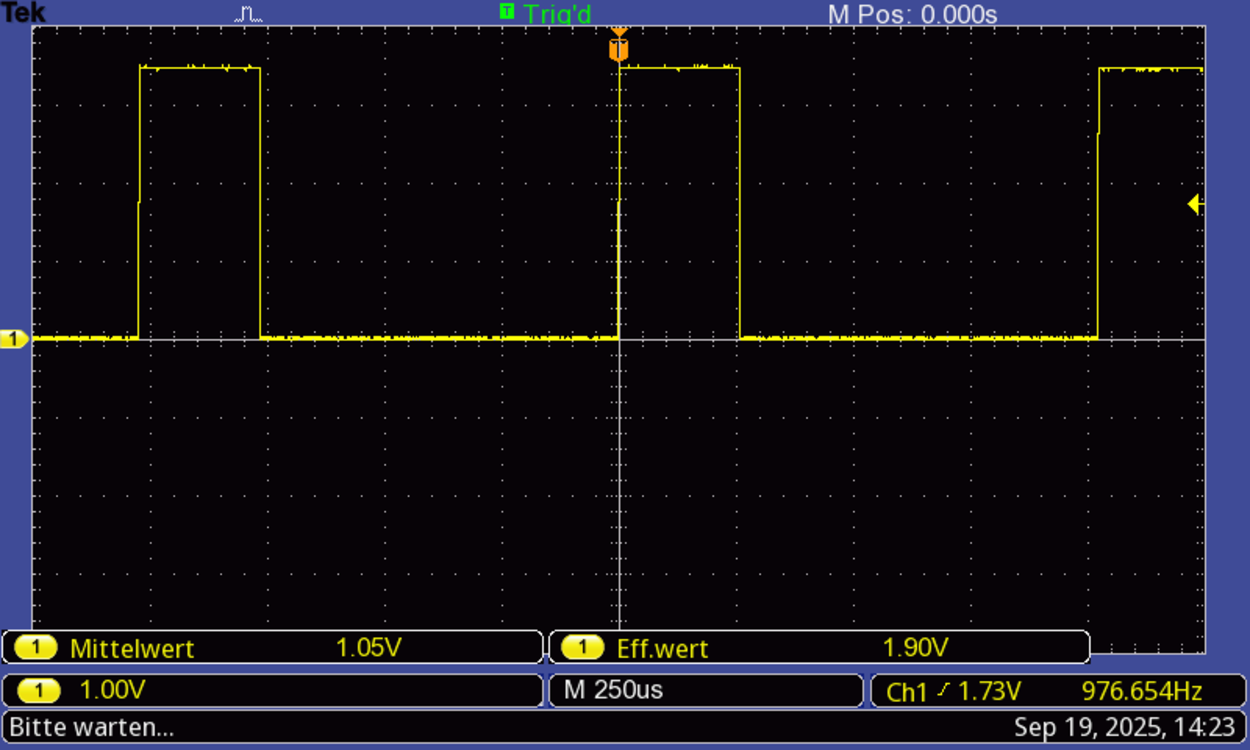
\includegraphics[width=0.45\textwidth]{img/25/Puls3/Puls25.pdf}
    \caption{Signal eines Pulses mit ungefährer Pulsbreite von 25\%.}
    \label{fig:sp_25}
\end{figure}

Wir übernehmen dabei die \hyperref[eq:f_3]{Ungenauigkeiten (\ref*{eq:f_3})} von Signal 1, da wir dieselbe Div-Größe haben. Auch die Fehler für die \hyperref[eq:f_avg]{mittlere Spannung (\ref*{eq:f_avg})} und die \hyperref[eq:f_eff]{Effektivspannung (\ref*{eq:f_eff})} werden von oben übernommen.
Somit kommen wir für die berechnete Mittelspannugn des zweiten Signals auf ein gesamt Ergebnis von:
\begin{equation}
    \boxed{
        U_{avg,r,2} = (0,878 \pm 0,019) \, V
    }.
\end{equation}

Und für die Effektivspannung:
\begin{equation}
    \boxed{
        U_{eff,r,2} = (1,73 \pm 0,04) \, V
    }.
\end{equation}

Auch hier wollen wir die signifikanten Abweichungen bestimmen:
Für die mittelre Spannung kommen wir auf eine Abweichung von
\begin{equation}
    \frac{\left| U_{avg,2} - U_{avg,r,2}\right|}{\sqrt{(\Delta U)^2 + (\Delta  U_{avg,r,2})}} = 2,17\sigma,
\end{equation} 

und für die Effektivespannung zu einem Wert von
\begin{equation}
    \frac{\left| U_{eff,2} - U_{eff,r,2}\right|}{\sqrt{(\Delta U)^2 + (\Delta  U_{eff,r,2})}} = 1,96\sigma.
\end{equation} 


% ////////////  Aufgaben Wechsel ////////////
\section{Aufgabe 4: Koaxialkabel}
Zu letzt soll die Länge des Koaxialkabels bestimmt werden. Am Ende des Kabels war eine Box mit drei möglichen Einstellung angebracht, die Auswirkung auf das Signal haben, welches durch das Koaxialkabel geleitet wurde: >>offen<<, >>zu<< und >>R<<.

\begin{figure} [h!]
    \centering
        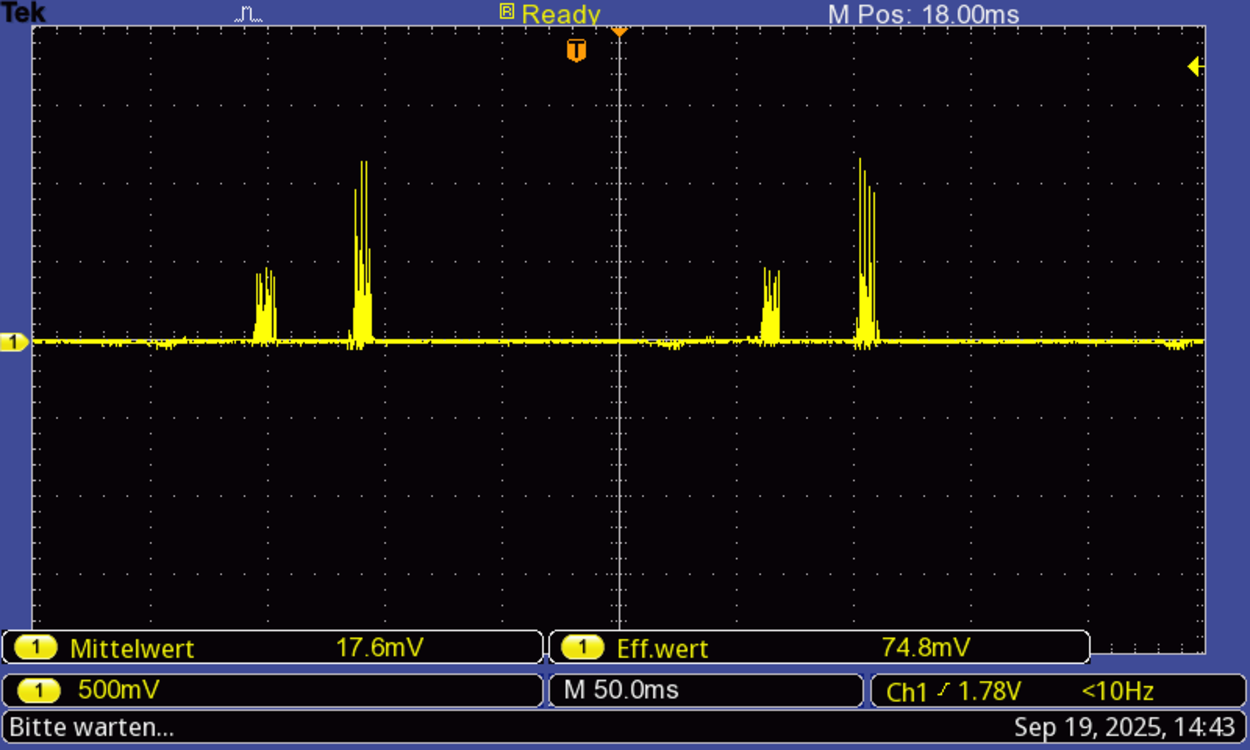
\includegraphics[width=0.45\textwidth]{img/25/Koaxial4/Koaxial-Kabel-offen.pdf}
    \caption{Signal (rausgezoomed) bei Einstellung >>offen<<}
    \label{fig:koax1}
\end{figure}

\begin{figure} [h!]
    \centering
        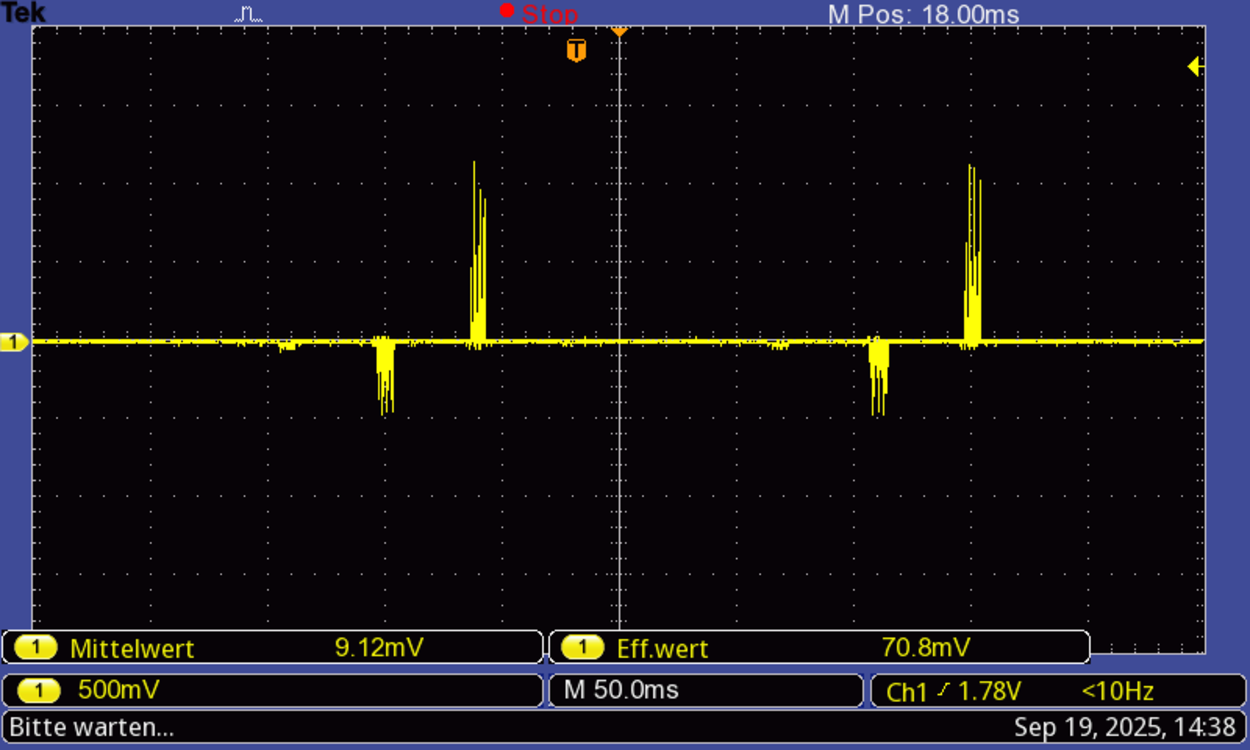
\includegraphics[width=0.45\textwidth]{img/25/Koaxial4/Koaxial-Kabel-zi.pdf}
    \caption{Signal (rausgezoomed) bei Einstellung >>zu<<}
    \label{fig:koax2}
\end{figure}

\subsection*{Über die gemessene Zeit}
Für die Zeitmessung bei offen und geschlossen (es ist derselbe Zeitwert) kamen wir auf eine Messung von:
\begin{equation}
    t = 188 ns.
\end{equation}

Wir haben dabei ein Div-Grid von $500mV \times 100ns$. Der zeitliche Fehler liegt damit bei
\begin{equation}
    \Delta t = 6,3 ns.
\end{equation}

Der Impuls hat sich mit 66\% der Vakuumslichtgeschwindigkeit bewegt. Die Länge des Kabels berechnet sich via:
\begin{equation}
    L = 0,66c \cdot \frac{1}{2} t.
\end{equation}

Setzen wir unsere Werte ein, so kommen wir auf
\begin{equation}
    \underline{
        L = 18,599 m
    }.
\end{equation}

Die Unsicherheit lässt sich via \hyperref[eq:gauss_fehlfortpflanzung]{Gauß'scher Fehlerfortpflanzung (\ref*{eq:gauss_fehlfortpflanzung})} bestimmen:
\begin{equation}
    \Delta L = 0,66c \cdot \frac{1}{2} \Delta t.
\end{equation}

Somit kommen wir auf eine Ungenauigkeit von:
\begin{equation}
    \underline{
        \Delta L =  0,623m.
    }
\end{equation}

Somit hat das Kabel eine Länge von
\begin{equation}
\boxed{
    L = (18,6 \pm 0,6) \, m
}
\end{equation}

\begin{figure} [h!]
    \centering
        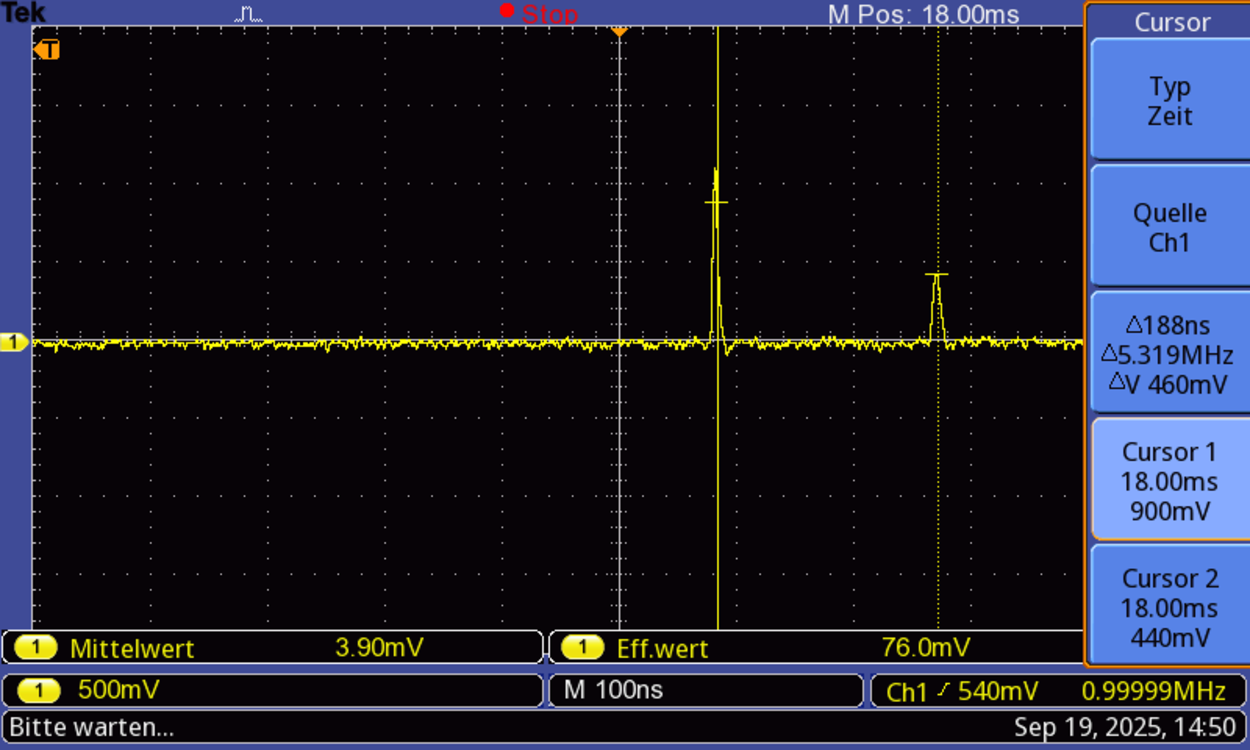
\includegraphics[width=0.45\textwidth]{img/25/Koaxial4/Koaxial-Kabel-Zoom.pdf}
    \caption{Signal für Zeitmessung}
    \label{fig:koax3}
\end{figure}

\subsection*{Über den gemessenen Widerstand}
Es lagen Voltmeter aus, um den Widerstand zu messen. Dafür wurde an der Box am Ende des Kabels auf >>R<< gestellt und an dem Drehrädchen solange gedreht, bis der eine Puls (der rechte) kleinst möglich war. ALso so nah wie möglich bei 0V.
Somit ließ sich über das Voltmeter dann der eingestelle Widerstand der Box bestimmen. Dieser lag bei:
\begin{equation}
    R = 38,3 \Omega.
\end{equation}

Die Ungenauigkeit des Ohmmeters liegt hierbei bei $1\Omega$. Das ausliegende Koaxialkabel ist ein RG58 Kabel, mit $50\Omega$ Wellenwiderstand. 
Wenn die Reflexion verschwindet, dann ist der gemessene Widerstand gleich dem Kabelwellenwiderstand. Berechnen wir die signifikante Abweichung:
\begin{equation}
    \frac{\left| 50 \Omega - 38,3 \Omega  \right|}{1 \Omega} = 11,7\sigma.
\end{equation}

\begin{figure}[h!]
    \centering
    
\includegraphics[width=0.22\textwidth]{img/25/memes/Udssr.pdf}
    \caption{(Schlechte Doku-Wahl.)}
\end{figure}